\documentclass{article}
\usepackage{ShumanNotes}
\title{Homework 1: Welcome to ECE 111}
\author{Kevin Stine}
\date{Due October 4th @ 3 PM, 2012}
\setlength{\parindent}{0pt}
\pdfpagewidth 8.5in
\pdfpageheight 11in

\begin{document}
\maketitle

\section{Introduction}
My name is Kevin Stine and I was born in San Diego, California and have lived in the San Fransisco Bay Area for the majority of my life. I enjoy most not traditional sports such as wakeboarding, snowboarding, skateboarding, and golf. I am also very into music and can play the piano, clarinet, guitar, bass guitar, and ukulele with most of my focus on guitar. I enjoy hanging out with friends, exploring nature, and long moonlit walks along the beach. I'm here at Oregon State University to pursue my interest in electrical engineering and hope that my four years here are productive and a great experience. 
\centerimage{\includegraphics[width = 4in]{./shotgun.jpg} }{Skeet Shooting}{ImageLabel}\newline
\newline


\section{Defining Success}
\emph{Success is the achievement of something desired, planned, or attempted. After you put years and thousands of dollars into your 
college education, what do you want from your ECE degree?}
\newline
\newline
I'm pursuing ECE because I find the topic very interesting and have loved learning about computers and how they work from a young age. I want to take my interest in computers and take it a step further by learning everything I can that ECE has to offer. I want to be knowledgable in the subject and eventually want to return to Silicon Valley to work for a company such as Apple or Nvidia. 

\section{Word Processing}
\emph{The homework assignments in ECE 111 focus on using Latex to typecast a professional looking .pdf for each assignment.  What are the advantages of Latex compared to traditional WYSIWYG \footnote{http://en.wikipedia.org/wiki/WYSIWYG} word processors?  What are the disadvantages of using Latex?}
\newline
\newline
I think that Latex is a good way to make sure every student's assignments are the safe format to save the teacher time from having to sort through many different fonts and styles. It makes sense that everyone's assignments will look the same to save time, but there is also a slight learning curve associated with using a specific software. Everything is formated similar to HTML format so you can see the commands for each line and see how it will show up in the pdf. This can be slightly confusing to people that have never used this kind of format before and it would be much harder than Microsoft Word or another kind of text editor. 

\section{Microcontrollers}
Atmel Microcontrollers are a very inexpensive way to develop projects.  Every future project in ECE 111 will use an Atmel Microcontroller, the Atmel Tiny26.\newline
\emph{Lookup the cost of the Tiny26 Microcontroller from Digikey}\newline
\url{http://search.digikey.com/scripts/DkSearch/dksus.dll?Detail&name=ATTINY26L-8PU-ND}\newline
\underline{For a single unit the price is \$ 3.06}\newline
\newline
\emph{Look up a project on Youtube that uses an Atmel Microcontroller}\newline
What does the Atmel Microcontroller do for the project you researched?\newline
\newline
\underline{The Microcontroller powers a custom TIX-like clock}


\section{Microcontroller Packages}
Integrated Circuits, ICs, are made using many different types of packages. The Tiny26 in lab is a DIP , while the 5 volt regulator is in a TO-92 package. The ECE 272 CPLD uses a 44 pin QFP. The Droid X OMAP processor is a BGA package type with over 400 pins! \newline
\newline
\emph{Insert a picture for the DIP, TO-92, QFP, and BGA package types}\newline
\newline
This link might be helpful \newline
\newline
\url{http://en.wikipedia.org/wiki/Chip_carrier}\newline
\newline

\centerimage{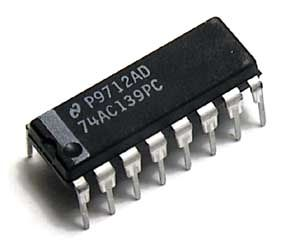
\includegraphics[width = 1.5in]{./dip.jpg} }{DIP Package}{ImageLabel}
\centerimage{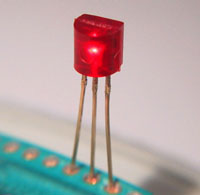
\includegraphics[width = 1.5in]{./to92.jpg} }{TO-92 Package}{ImageLabel}
\centerimage{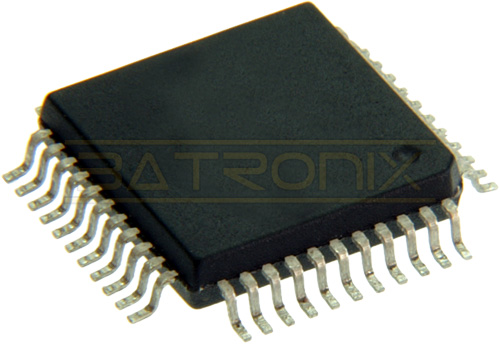
\includegraphics[width = 1.5in]{./qfp.jpg} }{QFP Package}{ImageLabel}
\centerimage{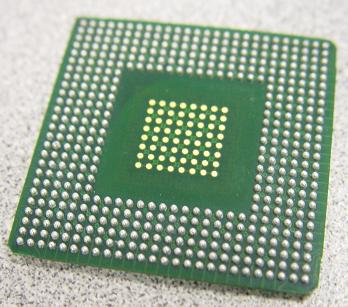
\includegraphics[width = 1.5in]{./bga.jpg} }{BGA Package}{ImageLabel}

\cfoot{ECE 111 Homework \#1}

\end{document}
